\documentclass{sigchi}

% Use this command to override the default ACM copyright statement (e.g. for preprints). 
% Consult the conference website for the camera-ready copyright statement.
\toappear{
	Submitted for review.
}

% Arabic page numbers for submission. 
% Remove this line to eliminate page numbers for the camera ready copy
\pagenumbering{arabic}


% Load basic packages
\usepackage{balance}  % to better equalize the last page
\usepackage{graphics} % for EPS, load graphicx instead
\usepackage{times}    % comment if you want LaTeX's default font
\usepackage{url}      % llt: nicely formatted URLs

\usepackage{textcomp}


% llt: Define a global style for URLs, rather that the default one
\makeatletter
\def\url@leostyle{%
  \@ifundefined{selectfont}{\def\UrlFont{\sf}}{\def\UrlFont{\small\bf\ttfamily}}}
\makeatother
\urlstyle{leo}


% To make various LaTeX processors do the right thing with page size.
\def\pprw{8.5in}
\def\pprh{11in}
\special{papersize=\pprw,\pprh}
\setlength{\paperwidth}{\pprw}
\setlength{\paperheight}{\pprh}
\setlength{\pdfpagewidth}{\pprw}
\setlength{\pdfpageheight}{\pprh}

% Make sure hyperref comes last of your loaded packages, 
% to give it a fighting chance of not being over-written, 
% since its job is to redefine many LaTeX commands.
\usepackage[pdftex]{hyperref}
\hypersetup{
pdftitle={Augmented Reality Tools for 
  the Creation of Physical Visual Arts},
pdfauthor={LaTeX},
pdfkeywords={augmented reality, projection mapping, drawing},
bookmarksnumbered,
pdfstartview={FitH},
colorlinks,
citecolor=black,
filecolor=black,
linkcolor=black,
urlcolor=black,
breaklinks=true,
}

% create a shortcut to typeset table headings
\newcommand\tabhead[1]{\small\textbf{#1}}

% End of preamble. Here it comes the document.
\begin{document}

\title{Augmented Reality Tools for \\ 
  the Creation of Physical Visual Arts.}

\numberofauthors{1}
\author{
  \alignauthor 1st Author Name\\
    \affaddr{Affiliation}\\
    \affaddr{Address}\\
    \email{e-mail address}\\
}

%% \numberofauthors{2}
%% \author{
%%   \alignauthor 1st Author Name\\
%%     \affaddr{Affiliation}\\
%%     \affaddr{Address}\\
%%     \email{e-mail address}\\
%%   \alignauthor 2nd Author Name\\
%%     \affaddr{Affiliation}\\
%%     \affaddr{Address}\\
%%     \email{e-mail address}\\
%% }



%% \begin{figure*}[th]
%% \centering
%% \includegraphics[width=85mm]{systempro.pdf}
%% \caption{Projection mapping resulting system.}
%% \label{fig:teaser}
%% \end{figure*}





\maketitle
 

\vspace{55mm}
\includegraphics[height=55mm]{teaser.pdf}

\begin{abstract}


We propose to empower the physical drawing creation with 
new spatial augmented reality tools. In order to do this, we created a
projection mapping system with paper tracking and touch input from a
depth camera. We created projection mapping tools to create drawings from
an empty canvas, an image or a 3D scene.

Construction lines are thin pencil strokes used to structure a
drawing. We push forward the limits of the use of construction lines
by enabling the creation of digital construction lines which can be
projected on any medium such as dark paper or wet paint.
Moreover, we show how image analysis tools
can be directly manipulated on paper to display the relevant
informations for drawing. 
We also enable the
visualization and manipulation of a cartoon shaded 3D scene. From these
manipulations, the user extracts a few images with different lighting
conditions. Each condition reveals relevant details, and they are
combined by the artist in one drawing. 
We conducted a user study to verify the usability and quality of our
user interface: it was found easy to use and led to higher quality
 perspective drawings. 

\end{abstract}



\includegraphics[height=55mm]{void.pdf}

\keywords{Spatial augmented reality, user interfaces, arts, interactive projection}
% \vspace{-0.15cm}


\category{H.5.1}{Information interfaces and presentation}{Information interfaces and presentation}
% \vspace{-0.15cm}

\terms{Design, Human Factors}
% \vspace{-0.15cm}

%% \keywords{
%% 	augmented reality; projection mapping; drawing; painting; non
%%         photorealistic rendering
%% }



\section{Introduction}

The creation of visual art is part of all Human history and is present
in every culture thorough history. It has a legacy of thousands of
years of materials and styles. The purpose of visual arts can be very
diverse such as religious, self-expression or for commercial
interests. 

Since the computer era, one can distinguish two types of visual art:
physical (\textit{e.g.} oil on canvas) and digital 
  (\textit{e.g.} jpeg file). The generation and edition of digital
images significantly changed our living environments: most photos,
newspapers and TV advertisements look ``perfect'', every details are
adjusted.  
This``perfection'' is inherent with the tools that created them. Every
error can be corrected with the undo-redo
commands. Moreover, the rendering and image edition tools
are extremely rich and they enable precise image creation.  
Conversely, with physical creation every mistake may leave a trace on
the final result. Or at least it will require more work to cover
it. There is no undo function in the physical world and the artist's
skills are tested on
every step of the creation. However, the expression is direct and
sensory rich: the paper's grain, the pencil's tip contact or the
paint's odor are also part the creation experience.

In this paper, we propose to enrich physical creation with digital
tools. These interactive tools are made to complement existing
techniques for the creation of physical visual arts. 
We propose to use computers for what they
are good at: image analysis and synthesis from line drawing to Non
Photorealistic Rendering (NPR). And to use Humans for what they are
good at: creativity, style and mistakes. 

%% TODO: refaire cette partie je pense...

We identified some limitations of existing traditional techniques, such as the
difficulty to trace guidelines over fresh paint or fragile mediums. 
Our first contribution is made to overcome this limitation. 
We propose a tool to create and edit
virtual construction lines which can be projected onto any medium. 
They can be general purpose construction lines: such as lines curves
and sketches. They can also be specialized such as construction lines
for perspective drawings. 
The second contribution of this paper is the possibility to 
to analyse a projected image with a touch-based interface. Consequently, 
only the details relevant for drawing are displayed. 
The third contribution enables the manipulation of a 3D
scene with NPR to create drawings. The user can capture the same view
of a scene with different light conditions: each light condition will
be used in different part of the final drawing. 
Finally, the last contribution of this paper is the evaluation of
the interactive projection mapping system we created for drawing. 
We evaluated its ease of use, and verified if digital construction
lines could replace physical construction lines. 


%% Similarly, we propose
%% to adjust the position and light conditions of a 3D scene in order to
%% render it with the relevant informations for the drawing. 

%% Our highly interactive tools also aid for the creation from rich media
%% such as images or 3D models. The artist can interactively process a 
%% part of an image in order draw it; he or she can also edit a 3D
%% rendering in order to use i during the creation process. 
 
%% Idée: Ajouter un paragraphe de motivations et limitations ? 

In this paper we first describe previous works on projection for drawing and
painting, and related works. Secondly, we describe the features of
our projection mapping system. Then, we introduce the digital
construction lines tools. After that, we show how one could use image
analysis, and edition to ease the drawing from any image. 
The next section is about NPR techniques for drawing. 
Finally, we describe the user experiment we conducted and
comment the results. 

%% conducted an user experiment to obtain formal
%% feedback on the quality and usability of our system. 


% Brief History, today's uses. 
%  

\section{Previous and Related Work}

%% A voir ce qu'on fait de ça...



\subsection{Projection for physical creation}

The camera obscura model has been used for
centuries~\cite{gernsheim1969history} as the first optical device to
project a planar image onto the real world. 
Nowadays equivalent are the art projectors, which enables the
projection of still images. They come with a wide variety of
resolutions and intensities.

In Projector-guided painting~\cite{flagg2006projector}, Flagg
\textit{et. al.} created a system dedicated to
painting. They proposed solutions to assist novices during the
whole painting process for: color mixing, brush stroke orientation,
and layering of the painting. They demonstrated that their system
successfully enabled novices to create high quality paintings. 
Our approach is much more generic and it focuses on the use of digital
tools not only for guiding, but also as part of the creation process
with the digital construction lines. It is
also designed to be highly interactive. %  and less intrusive. 


In PapARt~\cite{laviole:2012}, the authors proposed to project photos
to reproduce them on a paper with colored pencils and manipulate a
virtual 3D scene as a basis for drawing. They tested it on a few
subjects but did not provide any formal feedback. 
In this paper, we propose to extend this work on image projection with
image processing, and virtual 3D scenes with complete
examples. Furthermore, in this paper we propose a solution to trace digital
construction lines and a formal evaluation of the projection mapping
system and how it integrates with traditional tools. 
 
\subsection{Digital world integration}

%% Paper 
Paper is ubiquitous in our offices and homes and it may remain
for a long time~\cite{sellen2003myth}. 
The integration of physical paper with computing started
twenty years ago with the Digital Desk~\cite{wellner1993interacting}. 
It was further explored by Rekimoto
\textit{et.al.}~\cite{rekimoto1999augmented} and enriched with
tangible interfaces~\cite{ullmer2000emerging}. 

Moreover, this continuity is not limited to planar surfaces,
it can extend to any object: it is called Spatial Augmented Reality (SAR),
firstly created by Raskar \textit{et. al.}
\cite{raskar2001shader}. It enables to project
various
appearances on physical objects. Harrison \textit{et. al.} pushed this
integration forward to enable interactivity on self, or any surface with
OmniTouch~\cite{harrison2011omnitouch}. 

Our work is inscribed in the continuity of these works. Our goal is
to add new features to the physical world through computing. In this
paper we propose to use computing to overcome physical limitations and
assist the drawing by the use of NPR techniques~\cite{gooch2001non}. 

 
\subsection{Non Photorealistic Rendering}

The creation steps can be simulated
from analysis of the geometry of a scene~\cite{grabli2010programmable}. 
Many information can extracted from an image~\cite{haeberli1990paint}
or a 3D model~\cite{VBGS08} to create visually engaging NPR images. 
These rendering techniques can also be used during the creation
process. An example is Shadow Draw~\cite{leeshadowdraw} by Lee
\textit{et. al.}, which enables the rendering of probable strokes from
a database. 

In order to interactively create and project guidelines to assist
physical drawings we designed our own projection mapping system. 

%% ???
%% \subsection{Touch and tangible interfaces}
%% \cite{wilson2010combining}

\section{Projection Mapping System Design}

% Here -> constraints
\subsection{Design objectives}

We had two main objectives for the creation of the projection mapping system. The
first is the accuracy of the tracking-projection loop. Preliminary
studies showed that accuracy is a critical issue: a small error in
the calibration phase leads to projection errors. These errors lead to
deformations of the projection \textit{e.g.} a curve is drawn under
the projection, and then the drawing support is moved and the
projection does not match the curve any more.

The second objective is to enable direct interactions on the support 
without user instrumentation. Direct interaction is required because
most of the physical tools are direct: the line appears where the stroke
is done. It is an important factor for the perception of the system as
an augmentation of reality. 
In order to enable any kind of drawing medium in
terms of size and thickness we chose to use a vision-based touch
detection. Hence, a depth camera such as Kinect enables any scale and
provides enough precision for touch-based interactions. 

The system illustrated in Figure~\ref{fig:system} is completely
vision-based: it is composed of a procam (projector-camera) to detect
and project on paper and a Kinect to detect touch and hovering.
This kind of vision system scales well: it can be used for very precise
drawings as well as very large drawings with the same hardware
configurations. 

\begin{figure}[t!]
\centering
\includegraphics[width=85mm]{systempro.pdf}
\caption{Projection mapping system.}
\label{fig:system}
\end{figure}



\subsection{Additional tools}

%% The projection system is interactive with the touch input. However,
%% this kind of input does not provide active haptic feedback. 
%% Consequently, 

We integrated a
key-based interfaces on a small numeric pad with icons projected on
each key, as illustrated in Figure~\ref{fig:interface}. It is used for
menu selections. 
We also added an indirect pen input from a
 tablet. This input is used
for digital sketching over the physical drawing.

%% We created two dedicated tools for human body drawing, one uses the
%% hand pose recognition from Microsoft Kinect~\cite{shotton2013real}. The
%% Kinect is connected to another computer and the data is streamed via
%% the VRPN protocol using Faast~\cite{suma2011faast}. 

 

\section{Implementation details} 
 
  The system uses consumer products for hardware: a Microsoft
  Kinect (depth camera), Sony
  Playstation Eye (tracking camera), Logitech C905 (capture camera)
  and Vivitek Qumi Q2 (projector). We used a Wacom Bamboo Pen and Touch
  for pen input. 
  We used open-source software ProCamCalib~\cite{audet2010direct} by
  Samuel Audet to calibrate the cameras and projector. It enables us to
  achieve sub-pixel accuracy in average for the procam calibration. 

  The touch and hovering detection are custom-made and is similar to
  Wilson's in~\cite{wilson2007depth}.
  The marker tracking relies on ARToolKitPlus~\cite{wagner2007artoolkitplus}
  and most of the software uses OpenCV~\cite{opencv_library} and is coded
  with Processing~\cite{processing} and its numerous libraries.
  The lens distortions are handled by OpenCV (camera) and a dedicated
  shader (projector). The image analysis and synthesis shaders are coded in
  GLSL. 
  The softwares performed at cameras frame rates limits (30fps for touch,
  60fps for tracking) on a powerful laptop: Alienware m18x 2010 (core
  i7, GeFore580).
  All the inputs (touch and
  paper) are filtered using the 1\texteuro  ~Filter~\cite{casiez20121}. The
  ARToolkitPlus data were additionally filtered to block any translation
  inferior to 2cm while drawing, thus filtering the normal changes. 
  
  %% - TODO - 
  %% Placer ça à la fin ? 

  %% -- Deplacer\\
  %% During the experiment, the setup was in a virtual reality room, with
  %% a dedicated professional light setup. 
  %% The projection zone was  54cm by 34 cm with a 720p projector (5
  %% pixels per mm$^2$). The projected image will average a resolution of
  %% 650*460 pixels on a A4 paper sheet.\\
  %% -- Mettre une image avec ? 




%% \section{Initial Tools}

%% We created a collection of tools inspired from existing physical
%% techniques. 

%% Our digital tools have different advantages compared to
%% their physical equivalents. We focused into providing more comfort,
%% speed and cleanliness during the creation process. They are made to be
%% optionnal: they should not add new constraints to the tasks. 

%% % Intro : focus on the creation of digital tools to 
%% % complement the physical tools. 


%%   \subsection{Tracked Projection}

%%   Art projectors are fixed and the canvas is also immobile. We go
%%   beyond this limitation of art projectors by tracking the sheet of
%%   paper. With the tracking it is possible to move the canvas, and
%%   enables move the drawings during breaks. The projection
%%   requires a high quality tracking. Consequently, we chose to put
%%   markers all around the canvas in order to achieve a very good
%%   estimation of its orientation and high occlusion robustness.

%%   The projection can be used like an art projector: to copy the
%%   structure and colors of a drawing. In the next section we show
%%   other uses of interactive projection either to teach drawing or to
%%   support it. 


\section{Digital Construction Lines }

  Construction lines are lightly drawn lines that aid to draw the final
  stroke. They are used mostly in pencil sketches, and are generally
  required during the first creation steps. They are mostly
  used in pencil sketches because it uses the same tool for trials and
  final strokes. Consequently, the construction lines can be artifacts of the
  creation and may be part of the style. 

  It is a advised to beginners to draw as much construction lines as
  needed in order to obtain a good structure and maintain valid proportions.
  The creation of these construction lines is strenuous and 
  can be very difficult to erase. 
  Furthermore, for some creations it is impossible to use construction lines
  because the paper will get bruised from erasing, or remaining lines
  could not be deleted afterwards such as for watercolor. 
  For painting, the construction lines are drawn before
  painting. However, once it is covered it is impossible create new
  construction lines for the next layers. 

%% It is obviously
%%   impossible to create construction lines over paintings: once it is
%%   started there is no possible edition. 
  
  We enable the creation and edition of construction lines on any support by
  projecting digital construction lines. They can either replace or
  complement physical construction lines. 
  %% We propose two examples of dedicated construction lines,
  %% one for perspective drawings and the second is for character
  %% drawing. 

  %% The projection of digital construction lines enables automatic
  %% creation. 

  %% As they are projected, it is
  %% possible to use them in new contexts such as paint, and their
  %% deletion is not a problem either as they were never traced. 
  
  %% Inspired
  %% by courses from books ~\cite{cours-complet}\cite{dessinfacile}, we
  %% created a set of digital construction line creation tools. 
  %% We designed the user study to verify if digital construction lines
  %% could effectively replace physical ones. 

  \subsection{General purpose construction lines}

    The first set of construction lines tools are not specific to a
    type of drawing, they are illustrated in
    Figure~\ref{fig:line}~(a). The most simple structure we provide is a
    rectangular grid. 
    The grid is commonly used in drawings to copy, scale or deform an
    image. It provides a regular discretization of the space.
    In our implementation, the user can change the grid size, position
    and intensity and the grid size is displayed in millimeters. A
    grid is visible in Figures~\ref{fig:interface}~(a) and Figure~\ref{fig:group}~(d).

    \begin{figure}[!b]
      \centering 
      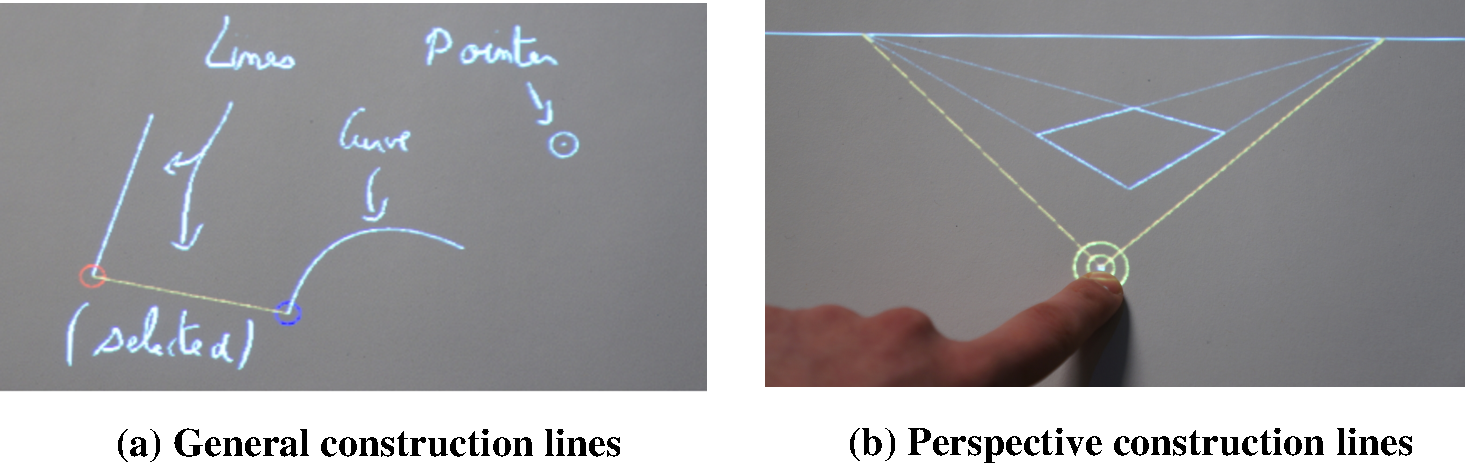
\includegraphics[width=85mm]{constructionline.pdf}
      \caption{General construction lines: lines, curves and sketches.}
      \label{fig:line}
    \end{figure} 

    The second construction line tool is line and curve drawing. The
    user can set the position of the two ends of a line. 
    He or she could add more lines, and snap the ends of
    lines together to fasten the creation of multiple lines or curves. 
    A line can be converted to a bezier curve, and two control points
    are added and can their positions can be adjusted.
    The last construction line tool is free drawing with the pen tablet
    input. This input is important for the structure of a drawing: the
    artist can sketch new shapes and see how it looks like directly on
    the drawing. The pressure controls the size of the projected strokes. 
    The users who tested it asked for more features, such as colors or
    layers. However, in this paper we focus on physical creation
    consequently we kept this interface very simple and raw. 
%% Further
%%     uses of the tablet is discussed in the future work section. 

    %% In the next section, we propose more specific construction line
    %% tools we created. 

  %% \subsection{Dedicated construction lines}

    %% We explore two tasks that require or benefit from construction
    %% lines: perspective drawing and character creation. 

    \subsection{Perspective construction lines}
    
    %% Perspective drawing requires specific construction lines, usually
    %% they originate from an object (such as a house) and goes towards
    %% the horizon at a vanishing point. 



%% We propose a set of tools to set the
%%     horizon and setup up the vanishing points. 

    %% One point perspective is when the viewpoint is facing an object,
    %% two point when objects are rotated from the user's point of view. 
    %% Three point perspective is for extreme cases where the viewpoint is very close
    %% to the ground or far above it, \textit{e.g.} such as skyscrapper
    %% drawings.
    A perspective drawing can have
    multiple vanishing points (up to three) depending on the point of
    view of the desired scene. 
    The user first sets the horizon and the vanishing points,
    then he or she can add new perspective points. 
    From each point a
    line which goes to each vanishing point is also created, as shown
    in figure~\ref{fig:line}~(b). We extended this tool to perspective
    quad drawing for two-point perspective.  
    From preleminary studies, this kind of automatic generation of
    construction lines seems to lead to faster drawings. 

    %% The perspective tool is
    %% richer than the general construction line tools. We removed it
    %% from user experiment, in order to have a shorter learning time of
    %% the user interface.


    %% \begin{figure}
    %%   \centering
    %%   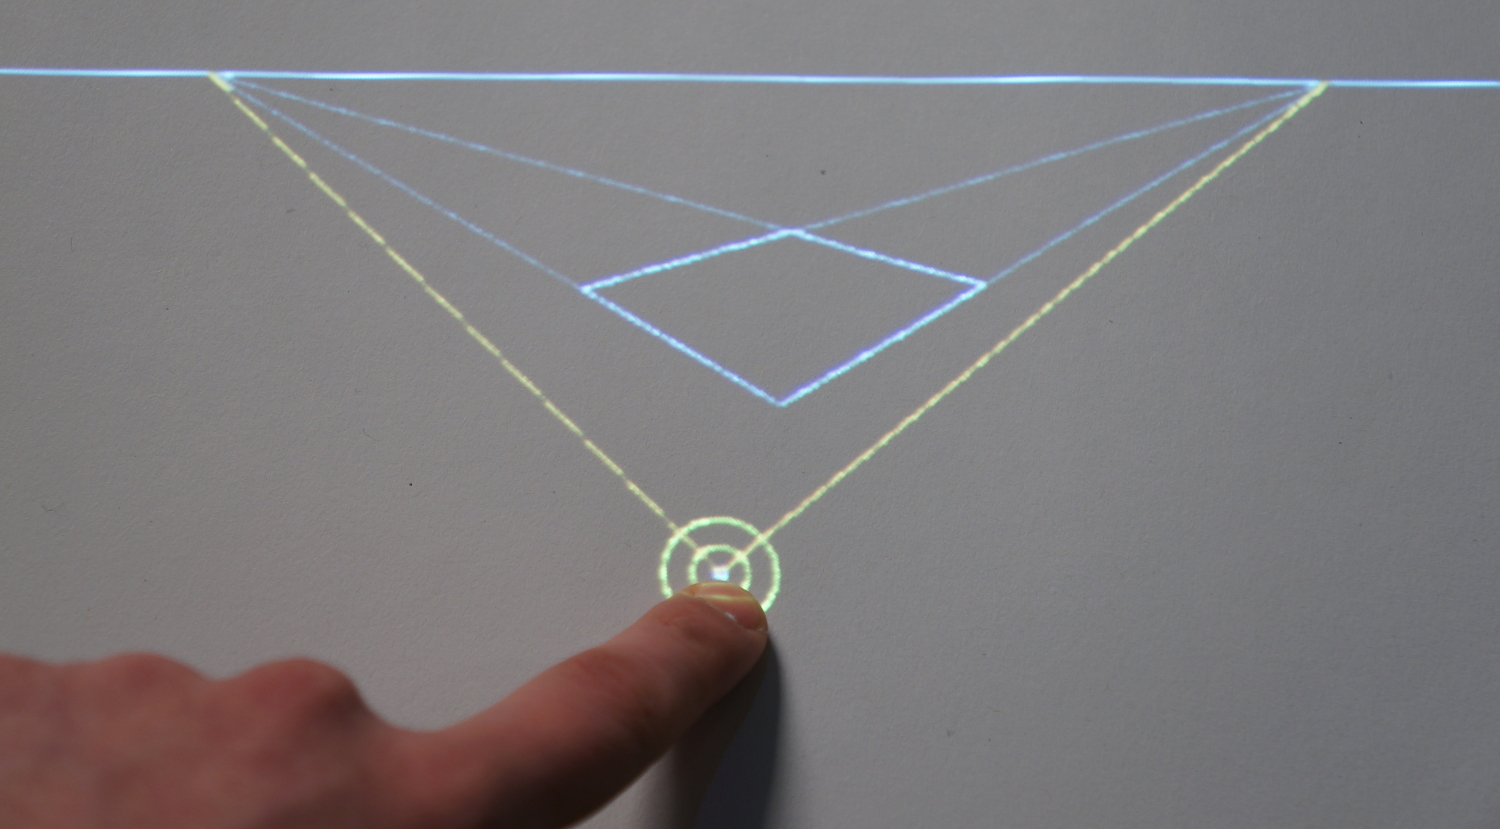
\includegraphics[width=75mm]{perspective2.JPG}
    %%   \caption{Construction lines dedicated to perspective drawing.}
    %%   \label{fig:vanish1}
    %% \end{figure} 
    

%%%%%%%%%%%%%%%%%%%%%%%%%%%%%%%%%%%%%%%%%%%%%%%%%%%%%%%%%%%%%%%%%%%%%%%%%%
    %%% Character drawing
%%%%%%%%%%%%%%%%%%%%%%%%%%%%%%%%%%%%%%%%%%%%%%%%%%%%%%%%%%%%%%%%%%%%%%%%%%


    %% \subsection{Character drawing}
 
    %% Character drawing is difficult to achieve because our perception
    %% of humans and more specifically faces is very good~\cite{puce1996differential}. 
    %% In this work, we focused on body proportions and pose. 

    %% %% For this, we created
    %% %% two tools: the first one is dedicated to novices. 

    %% We propose to project proportions for the whole body. These
    %% proportions changes with sex, age and strength. 
    %% These proportions varies between teaching books, in this work we followed the
    %% proportions rules from ``Figure Drawing for All It's
    %% Worth'' by Andrew Loomis~\cite{figuredrawing}. 
    %% The user can set
    %% the size of the construction lines, then he or she can choose to
    %% change strength or the age. The strength varies from 6.5 heads to
    %% 9 heads in height, with corresponding width. The age varies from 1
    %% year to 20 years according to Loomis' descriptions. 
    %% This tool constraints the pose of the character to a standing 
    %% position. It is a good exercise to learn how to draw limbs and
    %% memorize the proportions, as illustrated in Figure~\ref{fig:character}, however
    %% it is not enough for the creation of
    %% scenes full of characters. The next tool enables any pose for the
    %% character to draw. 


    %% \begin{figure}[!h]
    %%   \centering 
    %%   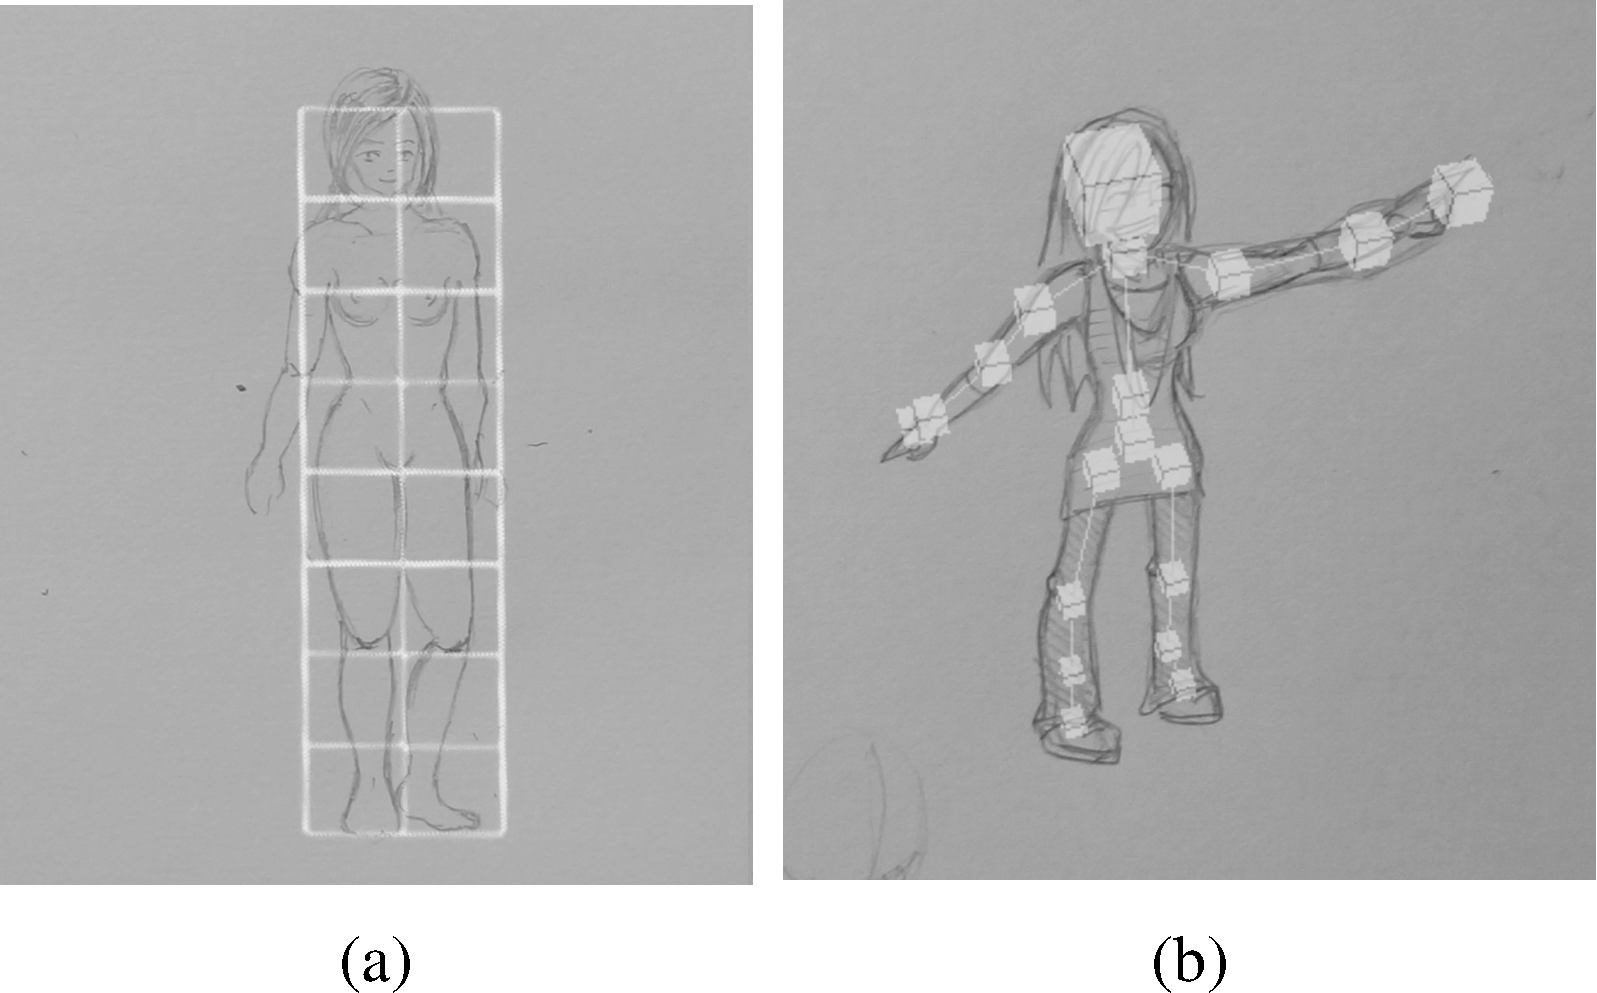
\includegraphics[width=85mm]{character.pdf}
    %%   \caption{Character drawing applications. Left: a grid
    %%     guides the character's proportions. Right: the 3D skeleton
    %%     from a Kinect guides the drawing.}
    %%   \label{fig:character}
    %% \end{figure}

    

    %% \subsubsection{Drawing from a model}

    %% The usual way to visualize a given pose is to use a mannequin
    %% (human or wooden),
    %% and put it into the desired pose. Here we propose to use a human
    %% model, and extract his or her pose using the skeleton tracking from 
    %% Kinect. The skeleton tracking is quite robust and allows a wide
    %% variety of poses. The 3D skeleton is projected on the paper and the
    %% point of view can be adjusted using the touch interface. 
    %% The user can then draw the character using the projected
    %% skeleton as illustrated in Figure~\ref{fig:character}. Further use
    %% of this tool and extensions are discussed in the future work
    %% section. 


%%%%%%%%%%%%%%%%%%%%%%%%%%%%%%%%%%%%%%%%%%%%%%%%%%%%%%%%%%%%%%%%%%%%%%%%%%
    %%% End of Character drawing
%%%%%%%%%%%%%%%%%%%%%%%%%%%%%%%%%%%%%%%%%%%%%%%%%%%%%%%%%%%%%%%%%%%%%%%%%%

    
In this section we presented new tools to help the artists during
their creation process. In the next section we propose new tools
using image analysis, and image synthesis to assist the creation
process.  


\section{Details from image analysis}
% \section{Step by step Drawings}

In this section we propose methods to assist the artist into deciding
which parts are important to draw for the final result. He or she can
adjust the algorithms and compose images to achieve the desired
result.  

%\subsection{Details from image analysis}

In previous works \cite{laviole:2012}, authors showed that the
projection of a photo can lead to a compelling drawing.
In these drawings, the user did copy the whole projected image. 
This lack of expression comes from the lack of interactivity.
The insight on which
details to draw or ignore requires training and experience. 
We propose to aid the artist on these decisions by the use of image
analysis techniques. 

\begin{figure}[h!]
  \centering 
  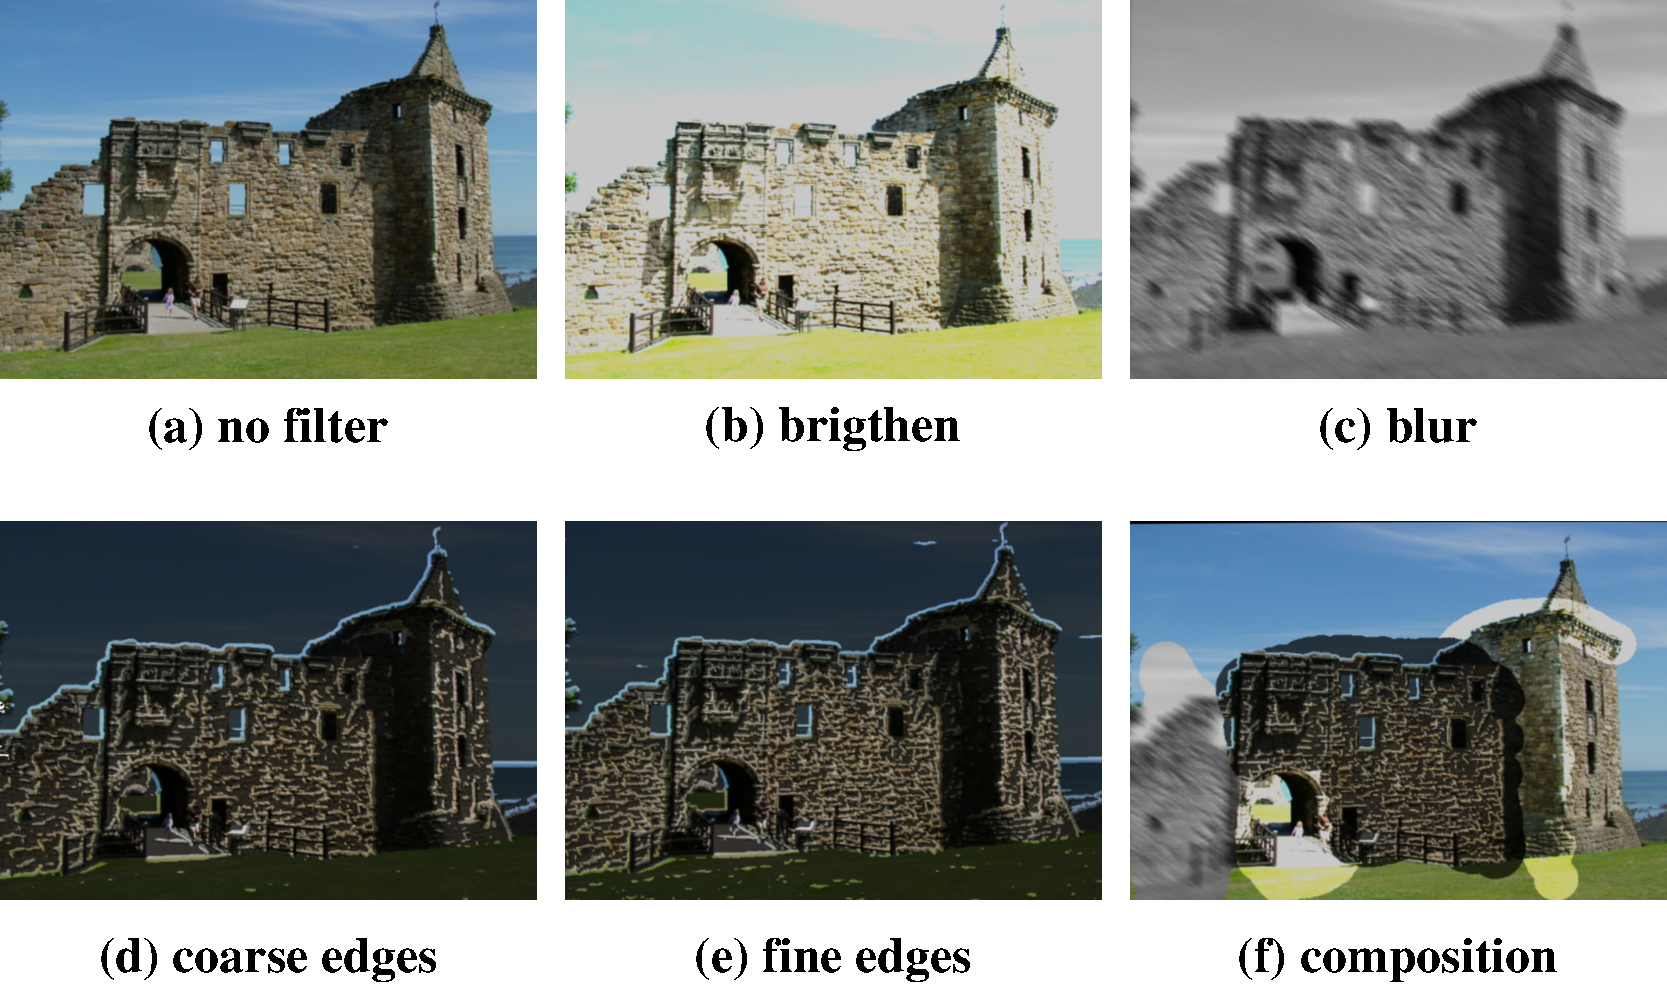
\includegraphics[width=85mm]{6maisons.pdf}
  \caption{ From a photo (a), the artist can directly apply image
    filters: brighten (b), blur(c), edge detection (d)(e), or a
    combination of them (f).}
  \label{fig:synthese}
\end{figure}
     

We propose to use three image enhancement methods, as illustrated in
Figure~\ref{fig:synthese}. The enhancements are applied directly on
the projection using the touch interface. They are displayed as
circles, the image (f) in Figure~\ref{fig:synthese} shows a
view during drawing. 

The first filter (b) brightens the projection on a given zone. It is
used to show more details from low-contrast zones. 
The second filter (c) blurs the image and makes it less bright. It is
used to set regions which are less interesting at a given time. 
The last filter (d)(e) is a derivates of gaussians filter. This filter
displays the edges (high gradient zones). The size of the analysis can
be adjusted to display different gradient sizes. Moreover, the
sensibility of the filter can also be adjusted to display more or less
informations. These filters are complemented control of the
projection's intensity.  This set of tools provide different point of
view on the same image; it is possible to use them to reveal details
that are hard or impossible to see without filters. 


We presented image analysis tools, in the next section we propose a
new use of NPR for drawing. 

%% TODO: encore une ou deux illstrations ?

%%  As the artist has to choose which
%% parts to use for the final drawing, he or she can
%% touch to blur the less interesting parts. 
%% Moreover, on the rest of the drawing it is possible to apply a
%% gaussian derivative filter to display contours of different sizes and
%% hide details. 

%% These image simplification are important for people want to learn to
%% draw. Here is it is done explicitly on an image, but skilled artists
%% trained their vision to only notice the relevent elements. 





 %%  The creation of a drawing requires many different steps. The first
%%   steps are the structuration of the drawing, \textit{i.e.} where each
%%   elements will be. As we explained before, our tools could help with
%%   the structure, and it can also help for next steps of the drawing
%%   process : adding details and shading. 


%%     The image analysis tools are numerous and dedicated to many
%%     applications, from healthcare to military uses. We propose to use
%%     some image filters to guide the drawing in steps following the
%%     natural drawing steps. 

%% %% TODO: Description of each step. Each one has one or two
%%     %% interaction. 

%% %% Black and white ?

%%     1. project the image with highly
%%     enhanced edges. The user have control on the influence of the
%%     edges. 
%%     2. Enhance finer details in the image. 


\section{Shading from image synthesis}



The suppression of useless details from a 3D scene to obtain a simpler rendering
is a difficult problem. It has been addressed in ``Where do people draw
Lines'' by Cole \textit{et. al.}~\cite{cole2008people}. 
Here we do not have the usual goals of NPR such as fully automatic and
temporally coherent rendering. 
Our approach here is to use multiple renderings to create one
drawing. Each rendered image highlight different details which are
recombined by the artist. 

%% We want to empower the artists with interactive control of the
%% rendered details. 
%% Consequently, he or she can display what is needed
%% for the drawing. 

Our example application is a hatching application using cartoon shading. 
The visualization metaphor we use is simple: the virtual object
is put on paper as if it was a physical object and the point of view
is fixed. 
The object can be moved, rotated and scaled using the multi-touch
interface. Its position is linked to the tracked piece of paper,
consequently the rendering is also controlled by the paper's position
and orientation. 

%% The scale is the only
%% non-physically plausible operation we allow on the model. 


%% Consequently the point of
%% view can also be adjusted by moving the piece of paper. 

%% \begin{figure}[!h]
%%   \centering 
%%   \includegraphics[width=85mm]{synthese.pdf}
%%   \caption{The user can use the paper to change the objects point of
%%     view (a)(b). He or she can also use the touch interface to rotate,
%%   scale or translate it (c)(d). Finally the light can be placed (e)(f).}
%%   \label{fig:multi-touch}
%% \end{figure}
    
\begin{figure*}[htb]
  \centering 
  \includegraphics[width=180mm]{touch1.pdf}
  \caption{User interface for the user study. The users could
    manipulate a grid (a), draw horizontal or vertical lines (b) and
    lines (c). The positioning of a line is either direct (b) or
    indirect (c).}
  \label{fig:interface}
\end{figure*}
  
 
Once the model is placed, its lighting is adjusted to show the
relevant details. 
The light's position is the user's hand position hovering over the
paper. He or she can take screenshots of different ligthing conditions 
to create the drawing, as illustrated in Figure~\ref{fig:hatching}
(a)(b)(c). The user set 3 lighting
conditions: one for each part of the body. Then, each captured image
is reprojected for the hatching phase. 
In this example, we propose to use three colors for the cartoon
shading, leading to three conditions : light hatching, heavy hatching
and no hatching. A result is shown in Figure~\ref{fig:hatching}~(d).
  
  

%% From a 3D
%% model, the user can choose a point of view using
%%  the multi-touch
%% interface. 
%% From this point of view, the scene is then rendered using a
%% simple toon shading. 

%% At this point the user can set the light
%% position by pointing and take screenshots of the different light
%% configurations. Each image will show different details. The final
%% drawing is a composition of the different lighting conditions as shown
%% in Figure~.. 



%% The source of the drawing can also be a 3D model, or a complete 3D
%% scene. Here for the sake of simplicity, we propose to use a 3D
%% model: the Stanford Bunny (cite ?). 

%% From a 3D model, the information is much richer than from an
%% image. Consequently, we can use more geometric and shading
%% information to guide the drawing. We propose to do Non
%% Photorealistic Rendering (NPR) to teach or ease the drawing. 
%% While classical NPR rendering algorithm focus on ``where'' to render
%% and ``how'' to render, here we only want the ``where'' information as the
%% user does the final result. 

%% In the example we created, we show how NPR rendering could be used
%% to teach hatching. We adapted a toon shading rendering technique
%% to decompose the drawing task in four different steps : 

%% %% List
%% 1. Draw the contour of the rabbit with a light pen. 
%% 2. Draw the first step of the hatching (darker regions)
%% 3. Draw the second step of the hatching (ligter regions)
%% 4. Create a fur texture for the whole rabbit. 
%% 5. Add some details if necessary. 

In the next section we evaluate the projection mapping system and some
of the tools we created through a user study. 



%% We proposed a set of new tools with example applications to create
%% physical drawings. The results are convincing on the usefulness of
%% these tools, consequently we conducted a user study to obtain more
%% data about the usability of the system and the new possibilities it
%% creates. 
 
%% In order to validate their use and the overall
%% usuability of projection to assist drawing, we conducted a controlled
%% user study.
\begin{figure}[!h]
  \centering 
  \includegraphics[width=75mm]{4lapins.pdf}
  \caption{The artist can choose different lighting conditions by
    hovering his or her hand over the scene. One
    for the ears (a), one for the head (b) and one for the body
    (c) to achieve one drawing (d).}
  \label{fig:hatching}
\end{figure}
    
\section{User evaluation}

We conducted a user study to evaluate the usability of the system. 
The first goal was to validate the perceived precision and quality of
the projection mapping system. The second goal was to check if our digital
construction line tools could effectively complement or even replace
physical construction lines. We did an independent measure evaluation
on 28 subjets on a perspective drawing. 


\subsection{Application}

  The application enabled the users to draw simple digital construction
  lines. The complete construction line tool solution was too rich for
  new users (none of them used the system before). 
  Consequently, we left only the most simple tools, which are more
  comparable to physical tools, consequently easier to learn. 
  The set of construction lines is illustrated in
  Figure~\ref{fig:interface}. 
  The users could display a grid (a),
  move it and change its scale. Additionally, they could create 
  horizontal and vertical lines (b), and lines by placing the two ends
  of it (c). The placement can be direct (b) or indirect (c). The
  users could switch between direct and indirect with a dedicated
  button. They could also be teleported to the closest point (with a
  .5cm threshold). 

  The user interface was displayed on a small numeric pad used by the
  non-dominant hand. Icons changed depending on the current mode and
  action, it is illustrated in Figure~\ref{fig:interface} on the left
  of each photo. We chose to
  use color codes to identify the ends of a line (red, blue), and the
  type of line (green).  Each line could be selected, edited and
  deleted using ``+'', ``-'' and ``del'' buttons of the numeric pad.


%% \begin{figure}[!h]
%%   \centering 
%%   \includegraphics[width=85mm]{numpad.pdf}
%%   \caption{User interface. May merge with the next figure}
%%   \label{fig:numpad}
%% \end{figure}
     


\subsection{Task}

   We chose to use an exercise from a pedagogical book on drawing
   entitled ``Dessiner pas a pas''~\cite{dessiner-ronin}
   (p.370-372). The task consists in a 
   step-by-step perspective drawing exercise of 17 construction lines
   which leads to a 11 lines house. It is made to be easy and it is
   extremely guided:
   each step contains a picture of the desired result and a short text
   describing how to achieve it. 
   We chose this guided task so that the drawings would be comparable
   to each other. Moreover it did not require any expertise in
   drawing, consequently the user's level in drawing did not interfere
   much during the experiment. 


   We divided the users in two groups, one group (BO: Book Only) uses the
   instructions, a H pencil, an eraser and a ruler. They had to
   follow the instructions, and we instructed them that all the lines
   that will be erased should be as light as possible to leave as less
   traces as possible. The BO group was composed of 6 male and 7
   female participants.
   The second group (P: Projection) had the same tools, and our system
   with the application described above. 
   They were instructed to avoid drawing construction lines as much as
   possible, in order to only draw the final strokes. The P group was
   composed of 7 female and 8 male participants. 

 \subsection{Participants}

   The participants were volunteers aged from 22 to 59
   ($\mu=29.9$). Most of them were novices in drawing, a few of them
   had a few drawing courses or draw at home, but none of them were
   trained professionals. We discarded two participants: one did not
   follow the instructions, and the second did not understood the
   concept of construction lines. 

\subsection{Apparatus}

  %% Most of the questions were on a 1-7 Likert, the other were
  %% open questions or they had to rate on a 1-7 scale. 


  Both groups had to take questionnaires before and after the drawing
  task. They were instructed to do the exercise at their own pace,
  although they knew the exercise was timed. 

  The BO volunteers were alone or in small groups in well-lit rooms
  with a large space to draw. Each had their own pencil, eraser, ruler
  and instructions. Once they were all ready, we asked for silence and
  gave them the written and oral instructions. 

  The P volunteers were in a virtual reality room with controlled
  light conditions. These constant light conditions were required to
  provide the same projection experience for every user. 
  The projection zone was  54cm by 34 cm with a 720p projector (5
  pixels per mm$^2$). The projected image averaged a resolution of
  650*460 pixels on a A4 paper sheet.

  Each participant had to begin with a training exercise which we timed
  to 10 minutes. One user required more time to learn how to use the
  interface. 


\section{Results}

\subsection{Drawing experience}
The three first questions of the questionnaire were common to both
groups. They were on a 1-7 Likert scale, with some space for comments. 
The questions and their results are displayed in Figure~\ref{fig:amusing}. 
The task was found easy ($\mu$=1.6) and amusing ($\mu$=2.07) by both
groups. Furthermore the felt as confident with digital lines as
with physical ones: BO $\mu$=2.07, P $\mu$=2.2. 
These similar results indicates that the experience of
drawing may not be altered, or at least that our system does not
negatively impact the drawing experience. 


%% \begin{itemize}
%%   \item (1) Did you find the experience amusing ?
%%   \item (2) Was the drawing task difficult ?
%%   \item (3) Were you confident before tracing ?
%% \end{itemize}



%% With these questions, they were able to add comments on the drawing
%% experience. The group 


%% We supposed that the projection could help to increase the
%% confidence before tracing. But, the task was easy and in both cases
%% they could place the ruler before tracing. 
%% Both groups were highly
%% confident: 
  

\begin{figure}[t!]
% \centering 
       \hspace{-5mm}
  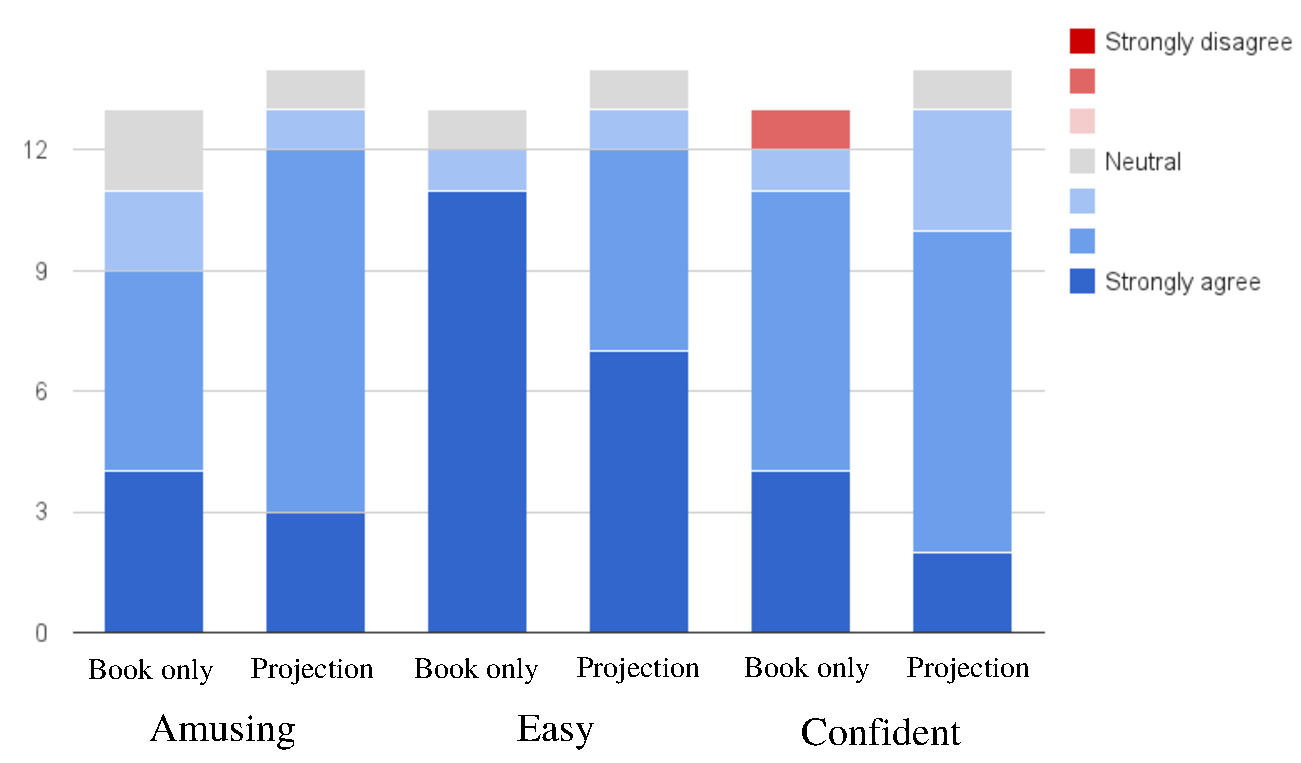
\includegraphics[width=95mm]{amusant.pdf}
  \caption{Subjective evaluation about the fun the users had, the ease
    of the task and their confident before tracing.}
  \label{fig:amusing}
\end{figure}

  
 \begin{figure*}[htp]
  \centering 
  
\includegraphics[width=180mm]{4dessins.pdf}
  \caption{Projection at the end of four drawings.}
  \label{fig:group}
\end{figure*}

 
\subsection{Observations on the projection}

The Projection group had five more questions about the user interface
and the overall experience with the projection. They were stated as
illustrated in Figure~\ref{fig:projection}.
The interface was designed to be simple and minimalist, so that the
users could focus on the drawing task without a long training
time. It was found easy to use by most users ($\mu$=2.3). 

We also colleced objective results on the interface use. 
They showed that the users did
not make many mistakes. The average creation number of horizontal or
vertical lines is 4.9 (SD=2.98) and standard line is 17.9 (SD=4.32). In 
the task they had to create 4 vertical lines and one horizontal, and
instructions from the book indicated the creation of 17 lines. 
The average number of keys pressed on the key pad was 185 (SD=61), for 13.5
(SD=4.4) actions per minutes. 

%% \begin{itemize}
%%   \item (4) Was the interface easy to use ?
%%   \item (5) Was the projection zone large enough ?
%%   \item (6) Was the projection inconveniant while drawing ?
%%   \item (7) Was the resolution high enough ?
%%   \item (8) Was the projection accurate enough ?
%% \end{itemize}

    \begin{figure}[htb]
%      \centering 
      \hspace{-5mm}
      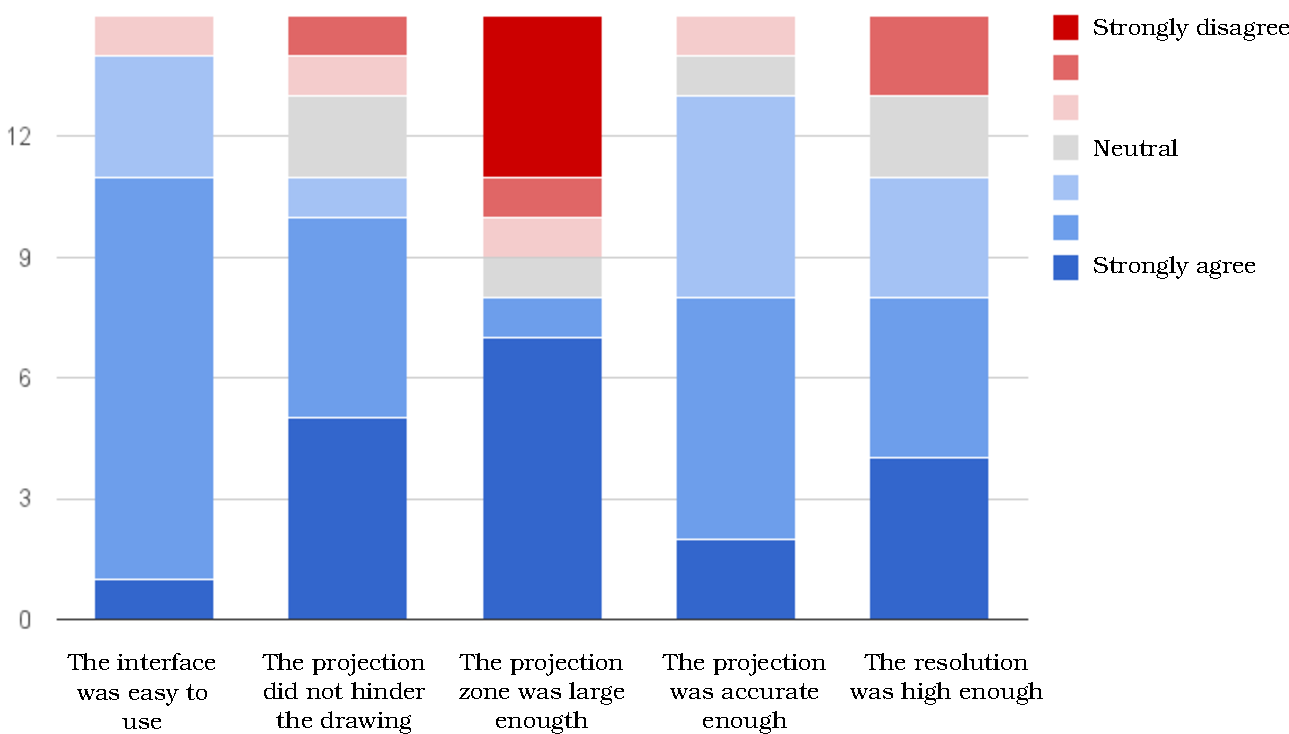
\includegraphics[width=95mm]{interfaceUse.pdf}
      \caption{Subjective evaluation of the augmented reality system.}
      \label{fig:projection}
    \end{figure}


The question about the size of the projection zone divided the users
in two groups. One group did not move the piece of paper, consequently
they never had any trouble with the size (8 users). The other group
changed their position more often and also the piece of
paper. Consequently, they encountered the projection's limits (7
users). 

The accuracy of the projection was found good enough ($\mu$=2.5).
However, some users reported that the definition of accuracy was not
completely clear to them. It was mixed with the displayed size of
construction lines. It is a positive point for us, it means that they
did not encounter any projection error. 
The perception of errors seemed dependent of the user's drawing
abilities (linear correlation coefficient : -0.395). 
The practice of drawing trains the visual system to see better and
better understand the shapes of objects. It can be an explanation of
the different perception of the imprecisions of the system. 
Trained users were also more sensible to the filtering we implemented.

The projection changes the perception of drawing, its intensity has to
be adjusted to the current light conditions with dedicated controls. 
With our controlled light conditions we managed to set projection
intensities that enabled a good visibility for both projection and
drawing. Most users found the projection more usefull than harmful
: $\mu$=2.5, SD=1.6. 


%% Most
%% users found the resolution accurate enough ($\mu$=2.7). 



%% Drawing without the necessity to move the canvas is part of the
%% learning process of drawing, to train the hand's agility.






\subsection{Drawing results}

We monitored the drawing duration, as we mentionned before the users were
instructed to draw at their own pace. The users without the projection
were faster: 10 minutes in average (SD=2.5) compared to 14 minutes (SD=2.9) with the
projection. The difference is statistically significant (p$<$0.05); it
was expected because the user interface was not performance oriented
but made to be easy to use. 
Moreover, the user had to take decisions on what kind of line to
project or use use the grid. An example of the variety of the uses of
the system is illustrated in Figure~\ref{fig:group}.
Another important observation is that most
users did more digital construction lines than instructed,
\textit{e.g.} in Figure~\ref{fig:group} (c) a hidden part of the roof is projected. 
%% We evaluated the drawings quality, as well as the use of the system to
%% objectively count the number of errors the users did. 


With our system, the drawing did have a few or no traces of erased
pencil. Moreover, we asked five persons in the lab to evaluate the
drawings to find errors (traces impossible to erase). The BO group had
a low number of errors: $\mu$=1.09, SD=1.30, and the P group even
less: $mu$=0.2 SD=0.38. 
The difference is statistically significant, the both values are very
low and the P users had to think more before tracing, and they spent
more time drawing. 
It would be interesting to evaluate more complex tasks to get a clear
observation on the error ratio. 

The overall results are good and they show that our system
successfully replaced the physical construction lines. We managed to
create a user interface to create digital construction lines easily. 
The drawings done without the projection were faster to do and most
all them had many traces of the construction lines. 
The time performance was not an issue for this user study, it quite
difficult to compare existing physical to new digital tools in terms
of training time because of the past experience of every user. 




%% We created three criterions to evaluate the resulting drawings, as
%% illustrated in Figure~\ref{fig:dessins1}. The first criterion is the
%% number of ``stars''. A ``star'' is small stroke of at least 0.5cm,
%% that have to be erased to obtain a ``perfect'' drawing. We did not
%% force the users from the group BO to erase all the stars, but all the
%% construction lines. The erasal of the stars could have diminished the drawing
%% time gap between the two groups. 
%% The second criterion to mesure the traces left of the construction
%% lines the ``Light lines''. These lines are
%% barely visible at 1 meter but easy to spot at a short distance. They
%% are construction lines that are not erased well, or traces on
%% the paper due to a heavy construction lines that have been erased. 
%% The last criterion mesures the errors done by the user. They are ``heavy
%% lines'': lines that were made to be final lines (bold strokes), but
%% needed to be erased. 

%% We gave these criterions to six different people in our research group
%% and the drawings for evaluation. All the drawings have been anonymized
%% and both groups were randomly mixed. We expected to have more ``stars''
%% and ``light lines'' without our system because of the traced
%% construction lines, and the results confirmed it. 


%% From these criterions we distinguish two types of drawings: ``normal''
%% and ``perfect'' drawings. Perfect drawings do not have any light nor
%% heavy line, we assume that the stars could be erased. The BO group had
%% 4 perfect drawings (30\%), one of it without stars. The P group had 9 perfect
%% drawings (60\%), none had stars. 
%% These results show that our projected construction lines successfully
%% replaced physical ones, and lead to cleaner drawings. 


 
%% \begin{figure}[!h]
%%   \centering 
%%   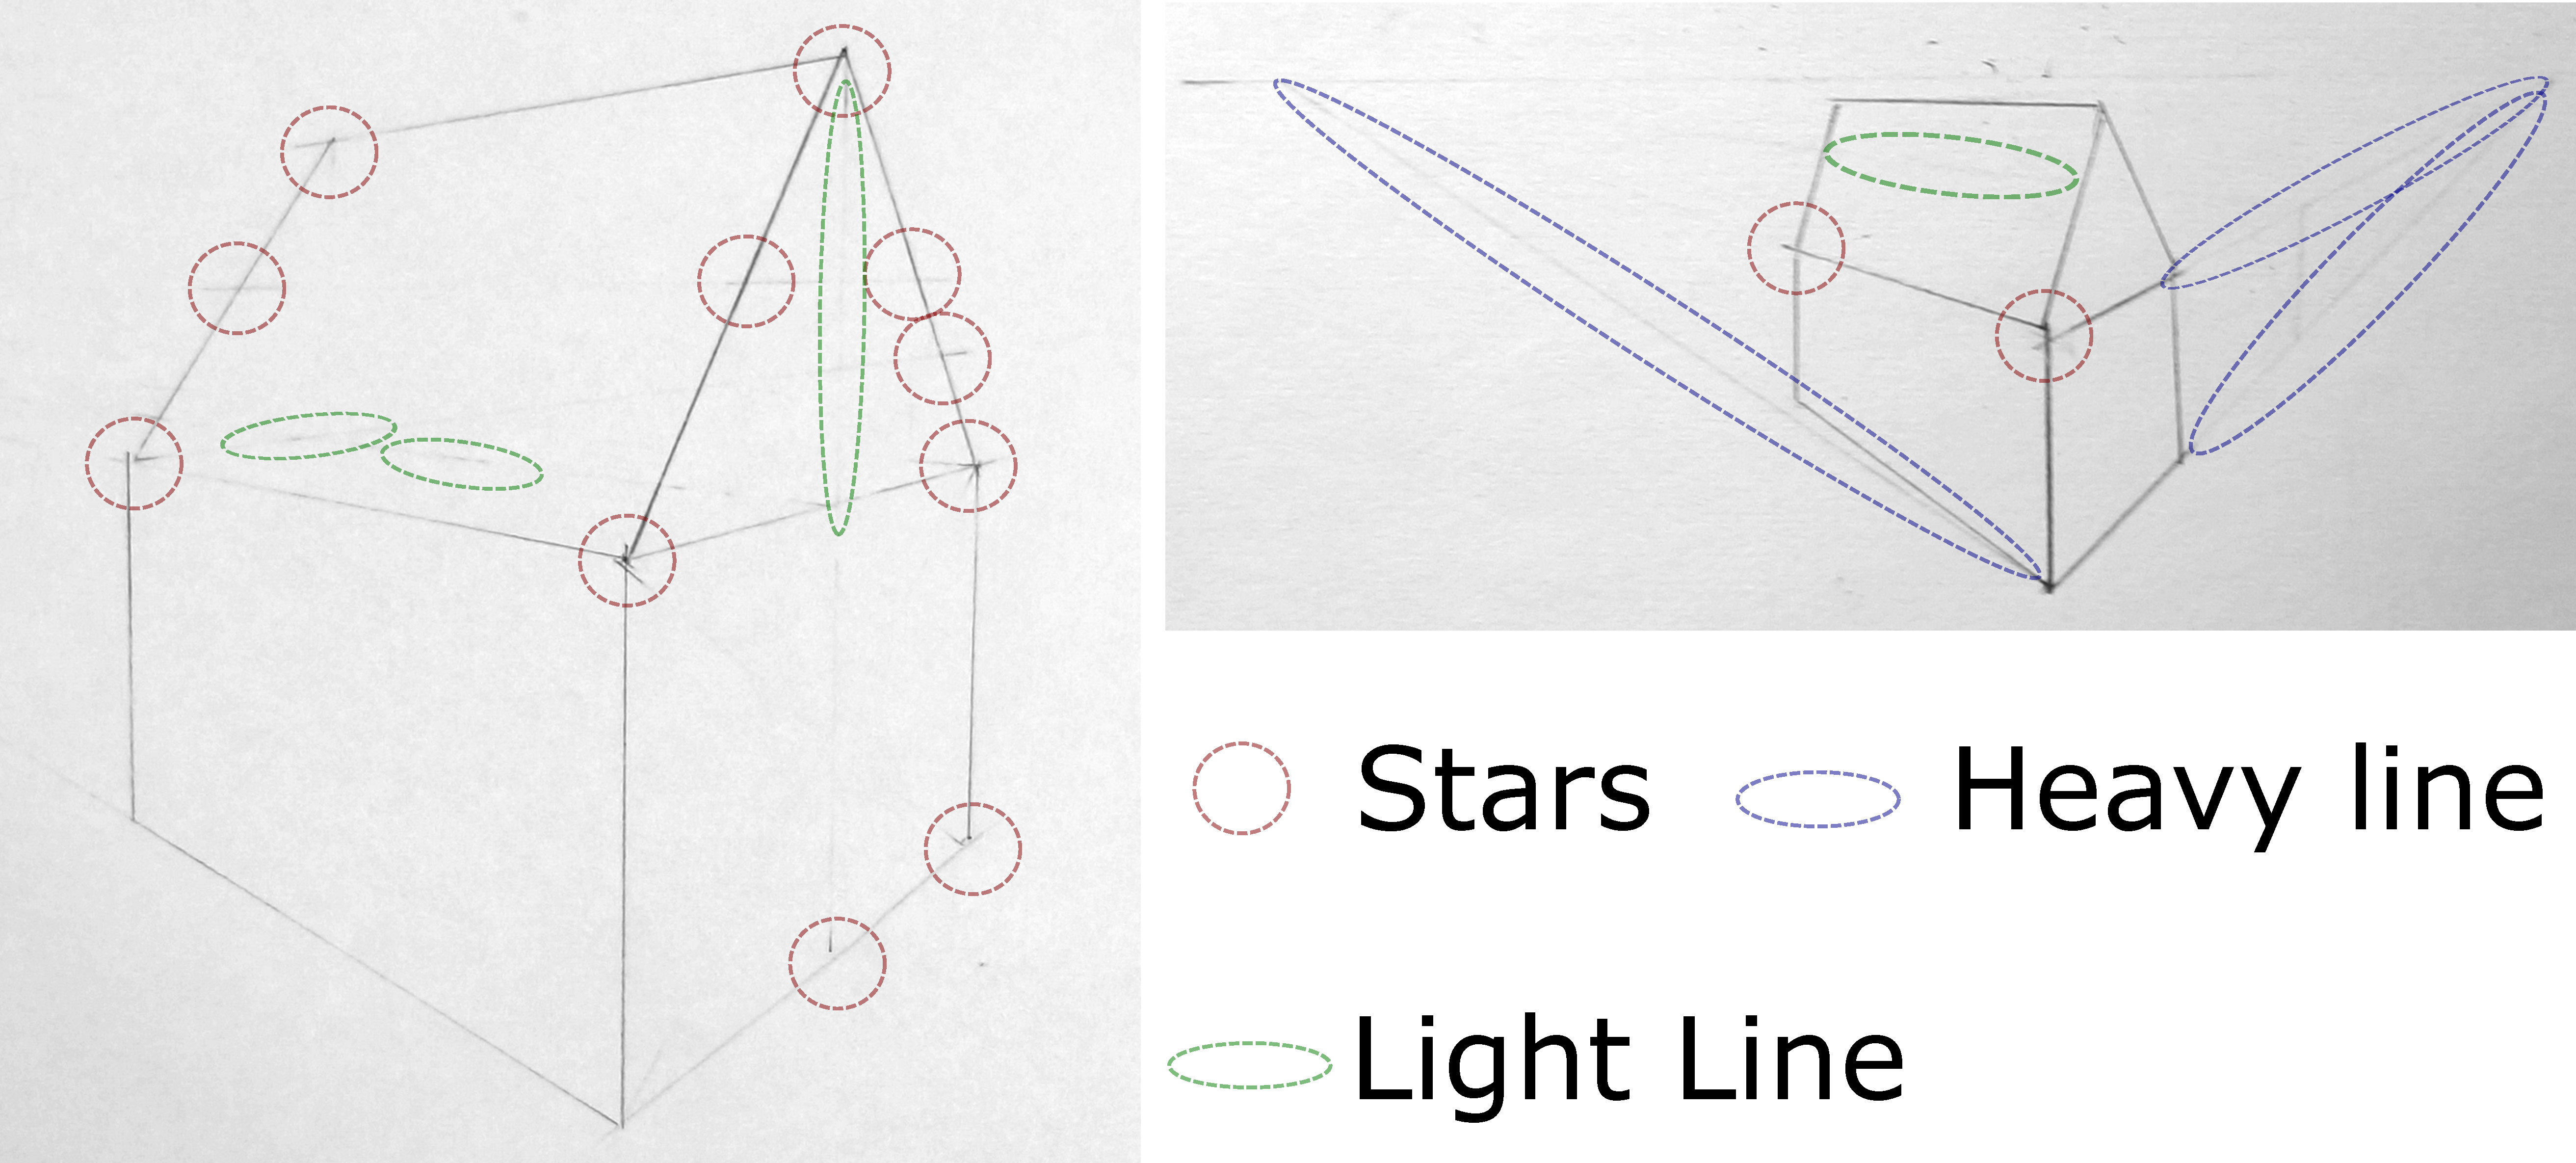
\includegraphics[width=75mm]{erreurs.pdf}
%%   \caption{Evaluation of the drawings.}
%%   \label{fig:erreurs1}
%% \end{figure}


%% \begin{figure}[!h]
%%   \centering 
%%   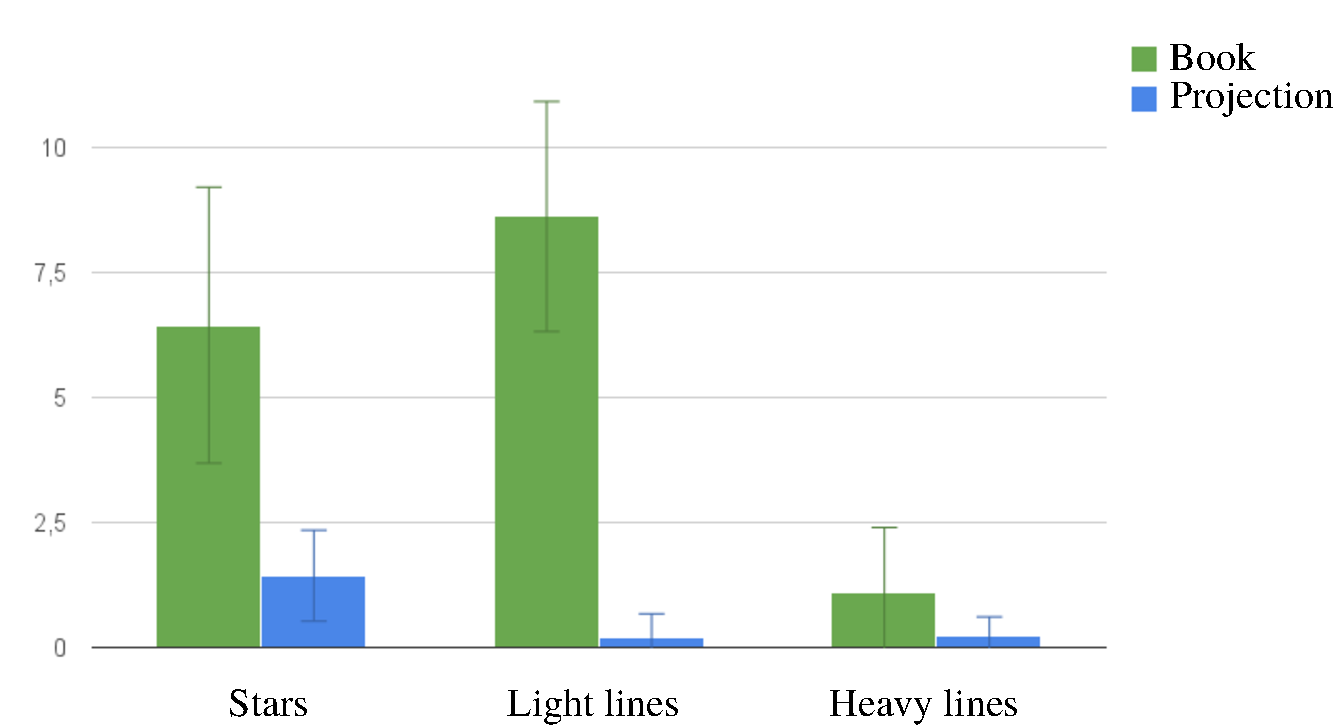
\includegraphics[width=75mm]{dessins.pdf}
%%   \caption{Objective evaluation of the drawings.}
%%   \label{fig:dessins1}
%% \end{figure}

%% TODO: illustration of the criterions. 

\section{Future work}

These tools are also well suited to teach the drawing: it is possible to
project the drawing instructions directly on paper. 
Moreover, the 
Kinect and the tracking camera can monitor the artist while drawing. We could
imagine a gamification of drawing courses, where not only the result counts
but also if the artist stayed still or moved a lot.

We presented one dedicated construction line tool for perspective. 
We started to develop more specific construction line tools for
character drawing. This is much more ambitious because of the
complexity of the human body. These construction line tools could
bridge the current gap between the NPR techniques we used and the
perspective tools. For example someone's pose is estimated using a
Kinect. Then the estimated skeleton is rendered using NPR and  placed
at the right scale using the perspective construction lines. 


%This work uses common techniques of image analysis and NPR. 

%% This kind of interactive rendering directly on the drawing medium may
%% diminish the bias on which line an artist would draw from an image. It
%% can be used to evaluate the results of NPR techniques that claim to be
%% close to man-made drawings. 


%% The creation of dedicated NPR techniques for drawing could make the
%% drawings creation much more easier and stimulate the artist's
%% creativity. 



\section{Conclusion}


In this paper we proposed three different techniques to ease the
drawing using projection mapping. The techniques can start from an
empty canvas, an image or a 3D scene. 
The first contribution is the use of digital construction lines to
structure a drawing. We proposed and evaluated a simple construction
lines tool and demonstrated an example of specific construction lines
for perspective drawing. 
Our second contribution is the use of image analysis directly on the
drawing medium. The artist can discard or enhance the different parts
of an image to make it easier to draw. 

The last method we proposed enables the creation of drawing from a 3D
scene. The scene is manipulated using the touch and tangible interface
and rendered with a NPR shading. The user can save screenshots of
different ligthing conditions to create a drawing where each part of
the model have a different illumination. 
 
%%  Consequently, he or she can create a drawing with a fake
%% shading highlight better details than a plausible shading. 

The user study we conducted showed that it is possible to use digital
construction lines to replace the physical ones. It enables the
creation of construction lines on any medium, such as dark or shiny
paper and wet paint. 
Finally, the overall user experience was good with our projection
mapping system and it encourages us to develop more complex and
audacious drawing tools. 


%% We also proposed to use an image to assist the drawing. We proposed to
%% apply image filters directly by touching the image. These filters can
%% hide or reveal details depending on the user's wishes. 


%% Tablet . 

%% Character drawing Model . 
\balance

% If you want to use smaller typesetting for the reference list,
% uncomment the following line:
\small
\bibliographystyle{acm-sigchi}
\bibliography{biblio}


\end{document}
